\documentclass{article}
\addtolength{\oddsidemargin}{-.875in}
\addtolength{\evensidemargin}{-.875in}
\usepackage[utf8]{inputenc}
\usepackage{color}
\usepackage{graphicx}
\usepackage{fancyhdr}
\usepackage{pseudocode}
\usepackage{verbatim}
\usepackage{listings}
\usepackage{rotating}
\usepackage[T1]{fontenc}
\usepackage[frenchb]{babel}
\usepackage{graphicx}
\usepackage{geometry}
\usepackage{hyperref}

\geometry{a4paper, top=2.5cm, bottom=2.5cm, left=3cm, right=2cm}

\begin{document}

\begin{titlepage}
    \begin{flushleft}
        
\includegraphics[width=0.2\textwidth]{./Visuels/Logo_INSA_Rouen.jpg}\par\vspace{1cm}
    \end{flushleft}
    \centering
    \vspace{1cm}
    {\huge\bfseries Projet Compresseur d'Huffman\par}
    \vspace{1cm}
    {\scshape\Large Groupe 11\par}
    \bigbreak
    \bigbreak
    \bigbreak
    \bigbreak
    \bigbreak
    \bigbreak
    \bigbreak
    \bigbreak
    
    \begin{minipage}{0.5\textwidth}
    \center
    
    \emph{Étudiants:}\\
    Tom \textsc{POGET}\\
    Basile \textsc{JORET}\\
    Haijiao \textsc{YU}\\
    Jean \textsc{ROUXEL}\\
    Mohamed Aziz \textsc{AYARI}\\
    \end{minipage}\\[2cm]

    \center
    \vspace{1cm}
    {\Large \emph{Date de Rendu}: 9 janvier 2024\par}
    \vspace{1cm}
    {\Large Enseignants Encadrants: \par}
    {\large N. Delestre et L. Vercouter\par}
    \vfill
\end{titlepage}

\pagenumbering{arabic}
\setcounter{page}{1}

\tableofcontents

\newpage
\section*{Introduction}
	Au cours de ce projet, nous avons eu l'opportunité de développer un compresseur d'Huffman. Afin d'y parvenir, nous avons tout d'abord mené une analyse descendante, puis créé les Types Abstraits de Données ArbreDeHuffman, CodeBinaire, FileDePriorité, Octet, Statistiques et TableDeCodage dont les spécifications, conceptions préliminaires et détaillées respectives se trouvent ci-dessous. Nous avons également créé un programme "principal" pour la compression mainCompression, un pour la décompression mainDecompression, et un mainGlobal qui se charge du choix entre les deux.
	
\newpage
\section{Analyse}
\subsection{Analyse Descendante}

\begin{sidewaysfigure}
    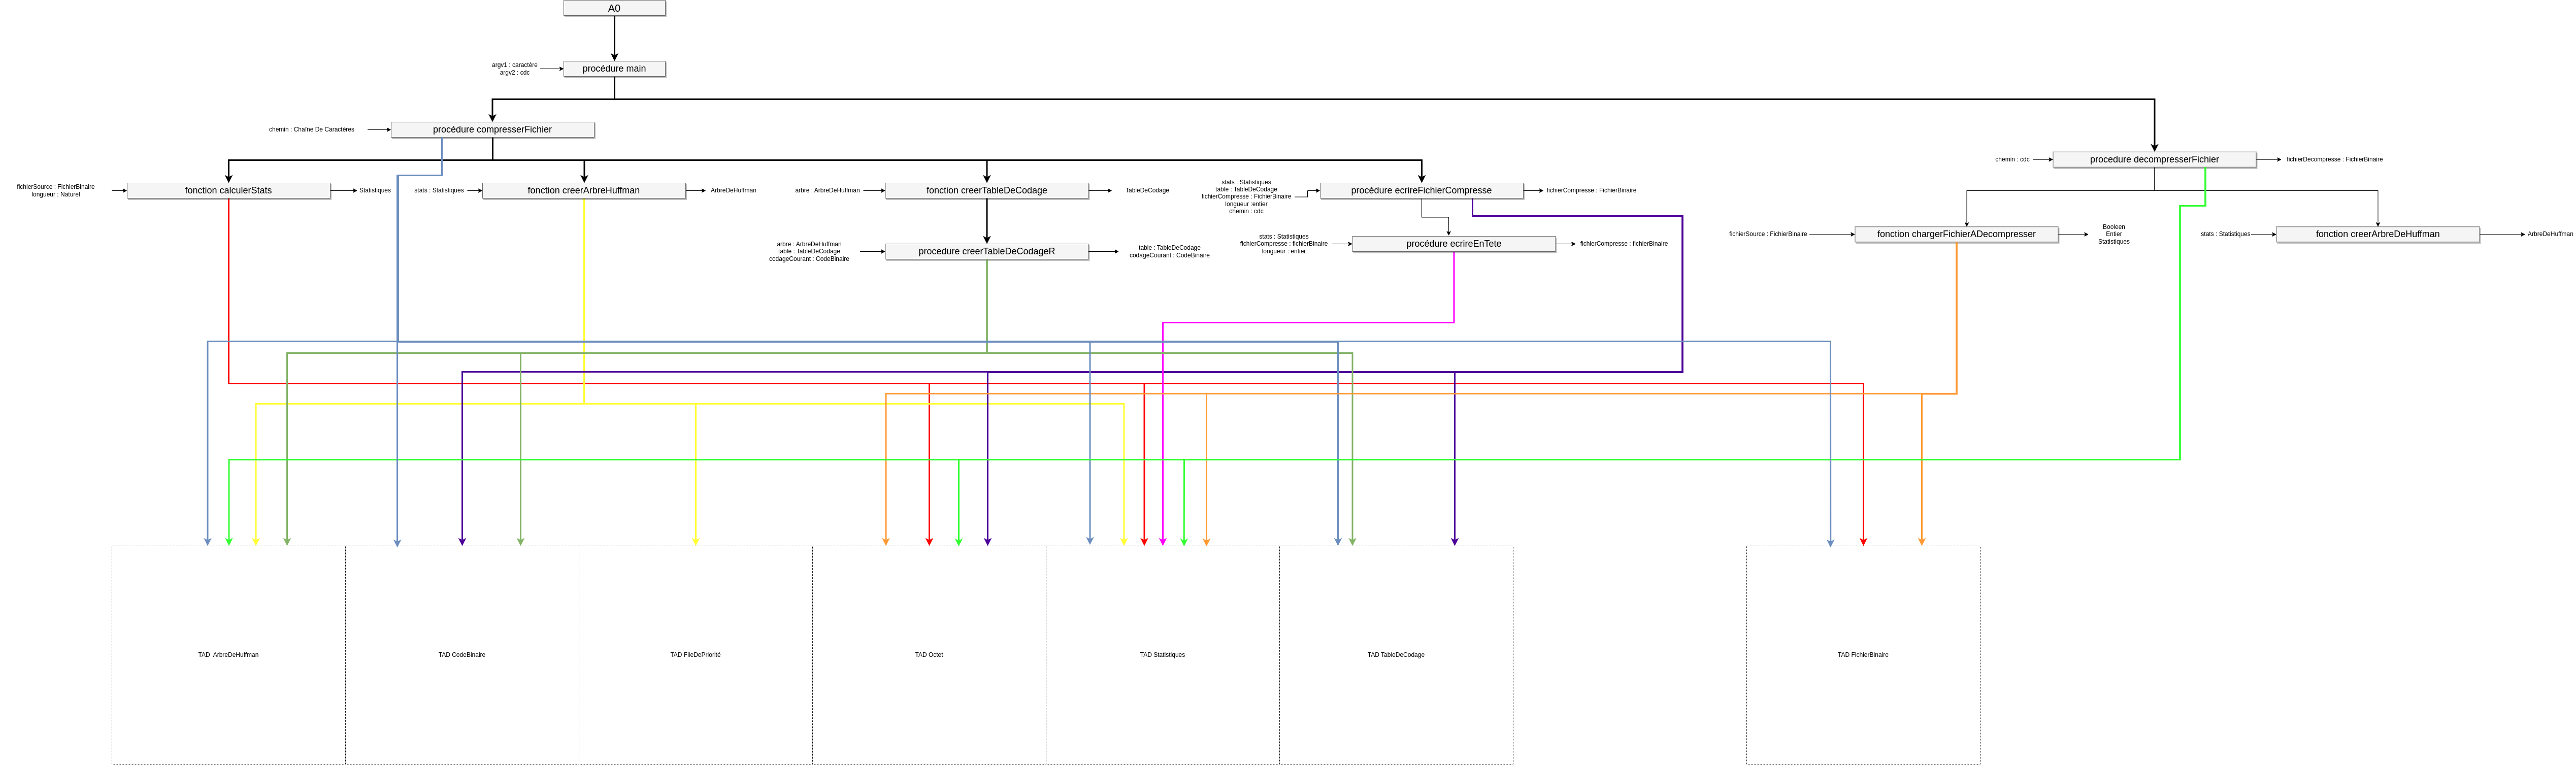
\includegraphics[scale=0.1]{./Visuels/Analyse_Descendante.png}
\end{sidewaysfigure}

\subsection{TAD}
\subsubsection{Arbre De Huffman}
	\begin{tad}
 \tadNom{ArbreDeHuffman}
 \tadParametres{Donnee (possède un ordre total)}
 \tadDependances{\booleen, \naturelNonNul}
 \begin{tadOperations}{obtenirDonnee}
 \tadOperation{feuille}{Donnee}{\tadParams{ArbreDeHuffman}}
\tadOperation{estUneFeuille}{\tadParams{ArbreDeHuffman}}{\tadParams{Booleen}}
 \tadOperationAvecPreconditions{obtenirFilsGauche}{\tadParams{ArbreDeHuffman}}{\tadParams{ArbreDeHuffman}}
\tadOperationAvecPreconditions{obtenirFilsDroit}{\tadParams{ArbreDeHuffman}}{\tadParams{ArbreDeHuffman}}
\tadOperationAvecPreconditions{obtenirDonnee}{\tadParams{ArbreDeHuffman}}{\tadParams{Donnee}}
\tadOperation{obtenirPonderation}{\tadParams{ArbreDeHuffman}}{\tadParams{\naturelNonNul}}
\tadOperation{ajouterRacine}{\tadParams{ArbreDehuffman, ArbreDeHuffman}}{\tadParams{ArbreDeHuffman}}
\end{tadOperations}
\begin{tadSemantiques}{longueur}
\tadSemantique{feuille}{crée un arbre de Huffman (feuille) à partir d'une donnée}
\tadSemantique{ajouterRacine}{rassemble deux arbres et calcule la pondération associée (somme des pondérations/données des deux sous-arbres)}
\end{tadSemantiques}
\begin{tadAxiomes}
\tadAxiome{estUneFeuille(feuille())}
\tadAxiome{non(estUneFeuille(ajouterRacine(ag,ad)))}
\tadAxiome{obtenirDonnee(feuille(d))=d}
\tadAxiome{obtenirFilsGauche(ajouterRacine(ag,ad)) = ag}
\tadAxiome{obtenirFilsDroit(ajouterRacine(ag,ad)) = ad}
\end{tadAxiomes}
\begin{tadPreconditions}{obtenirDonnee(a)}
\tadPrecondition{obtenirFilsGauche(a)}{non estUneFeuille(a)}
\tadPrecondition{obtenirFilsDroit(a)}{non estUneFeuille(a)}
\tadPrecondition{obtenirDonnee(a)}{estUneFeuille(a)}
\end{tadPreconditions}
\end{tad}

    
\subsubsection{Code Binaire}
	\begin{tad}
\tadNom{CodeBinaire}
\tadDependances{\booleen, \naturelNonNul, \naturel , Bit}
\begin{tadOperations}{obtenirElement}
\tadOperation{codebinaire}{}{\tadParams{CodeBinaire}}
\tadOperation{estVide}{\tadParams{CodeBinaire}}{\tadParams{Booleen}}\tadOperationAvecPreconditions{insererBit}{\tadParams{CodeBinaire, \naturelNonNul,Bit}}{\tadParams{CodeBinaire}}
\tadOperationAvecPreconditions{supprimerBit}{\tadParams{CodeBinaire, \naturelNonNul}}
{\tadParams{CodeBinaire}}
\tadOperationAvecPreconditions{obtenirBit}{\tadParams{CodeBinaire, \naturelNonNul}}{\tadParams{Bit}}
    \tadOperation{obtenirLongueur}{\tadParams{CodeBinaire}}{\tadParams{\naturel}}
\end{tadOperations}
\begin{tadSemantiques}{obtenirLongueur}
\tadSemantique{codeBinaire}{Crée un CodeBinaire vide}
\tadSemantique{insererBit}{Insère un bit a une position donnée}
\tadSemantique{obtenirLongueur}{Renvoie la longueur du CodeBinaire}
\end{tadSemantiques}
\begin{tadAxiomes}
\tadAxiome{estVide(codebinaire())}
\tadAxiome{non estVide(inserer(CB,i,bit()))}
\tadAxiome{supprimerBit(insererBit(CB,i,bit),i) = CB}
\tadAxiome{obtenirBit(insererBit(codebinaire(),0,bit),0) = bit}
\tadAxiome{obtenirLongueur(insererBit(CB,i,bit) = obtenirLongueur(CB)+1)}
\end{tadAxiomes}
\begin{tadPreconditions}{obtenirElement(l,i)}
\tadPrecondition{insererBit(CB,i,bit) : i $\leq$ obtenirLongueur(CB)+1}
\tadPrecondition{supprimerBit(CB,i)}{i $\leq$ obtenirLongueur(CB)}
\tadPrecondition{obtenirBit(CB,i)}{i $\leq$ obtenirLongueur(CB)}
\end{tadPreconditions}
\end{tad}
\subsubsection{File De Priorité}
	\begin{tad}

    \tadNom{FileDePriorite}
    \tadParametres{Element}
    \tadDependances{\booleen, \naturel}
    
    \begin{tadOperations}{fileDePriorite}
        \tadOperation{fileDePriorite}{}{\tadParams{FileDePriorite}}
        \tadOperation{estVide}{\tadParams{FileDePriorite}}{\tadParams{\booleen}}
        \tadOperation{inserer}{\tadParams{FileDePriorite, Element}}{\tadParams{FileDePriorite}}
        \tadOperationAvecPreconditions{defiler}{\tadParams{FileDePriorite}}{\tadParams{FileDePriorite, Element}}
        \tadOperationAvecPreconditions{obtenirElement}{\tadParams{FileDePriorite}}{\tadParams{Element}}
        \tadOperation{longueur}{\tadParams{FileDePriorite}}{\tadParams{\naturel}}
    \end{tadOperations}

    \begin{tadAxiomes}
        \tadAxiome{estVide(fileDePriorite())}
        \tadAxiome{non(estVide(inserer(f,e)))}
        \tadAxiome{longueur(fileDePriorite()) = 0}
        \tadAxiome{longueur(inserer(f, element)) = 1 + longueur(f)}
        \tadAxiome{defiler(inserer(fileDePriorite(), e1)) = fileDePriorite(), e1}
        \tadAxiome{obtenirElement(inserer(fileDePriorite(), e)) = e}
    \end{tadAxiomes}

    \begin{tadPreconditions}{defiler(f)}
    	\tadPrecondition{obtenirElement}{non estVide(f)}
        \tadPrecondition{defiler(f)}{non estVide(f)}
    \end{tadPreconditions}

\end{tad}
   
       
\subsubsection{Octet}
	\begin{tad}

    \tadNom{Octet}
    \tadDependances{\naturel, Bit}
    
    \begin{tadOperations}{modifierBit}
        \tadOperation{octet}{}{\tadParams{Octet}}
        \tadOperationAvecPreconditions{modifierBit}{\tadParams{Octet, \naturel, Bit}}{\tadParams{Octet}}
        \tadOperationAvecPreconditions{iemeBit}{\tadParams{Octet, \naturel}}{\tadParams{Bit}}
    \end{tadOperations}

    \begin{tadSemantiques}{modifierBit}
        \tadSemantique{octet}{creer un Octet qui contient 8 bits}
        \tadSemantique{modifierBit}{modifier l'ième bit de l'Octet}
        \tadSemantique{iemeBit}{retourne l'ième bit de l'Octet}
    \end{tadSemantiques}

    \begin{tadAxiomes}
        \tadAxiome{iemeBit(modifierBit(o,u,b),i) = b}
    \end{tadAxiomes}

    \begin{tadPreconditions}{modifierBit(o,i,b)}
        \tadPrecondition{modifierBit(o,i,b)}{i $\leq$ 8}
        \tadPrecondition{iemeBit(o,i)}{i $\leq$ 8}
    \end{tadPreconditions}

\end{tad}
\subsubsection{Statistiques}
	\begin{tad}

\tadNom{Statistiques}
\tadDependances{\booleen, Octet, \naturel, \naturelNonNul}

\begin{tadOperations}{obtenirValeurs}
	\tadOperation{statistiques}{}{\tadParams{Statistiques}}
	\tadOperation{ajouter}{\tadParams{Statistiques, Octet}}{\tadParams{Statistiques}}
	\tadOperationAvecPreconditions{retirer}{\tadParams{Statistiques, Octet}}{\tadParams{Statistiques}}
	\tadOperation{estPresent}{\tadParams{Statistiques, Octet}}{\tadParams{\booleen}}
	\tadOperationAvecPreconditions{obtenirOccurrence}{\tadParams{Statistiques, Octet}}{\tadParams{\naturelNonNul}}
	\tadOperation{obtenirOctets}{\tadParams{Statistiques}}{\tadParams{Liste $<$Octet$>$}}
	\tadOperation{obtenirOccurrences}{\tadParams{Statistiques}}{\tadParams{Liste $<$\naturelNonNul$>$}}
	\tadOperation{nbElements}{\tadParams{Statistiques}}{\tadParams{\naturel}}
\end{tadOperations}

\begin{tadSemantiques}{obtenirOccurences}
	\tadSemantique{statistiques}{Crée un tableau de statistiques vide}
	\tadSemantique{obtenirOctets}{Obtient la liste des octets présents dans les Statistiques (soit dont le nombre d'occurrences est strictement supérieur à 1)}
	\tadSemantique{obtenirOccurences}{obtient la liste des occurrences présentes dans les Statistiques, dans l'ordre des clés (Octets)}
\end{tadSemantiques}

\begin{tadAxiomes}
	\tadAxiome{non estPresent(statistiques(), o)}
	\tadAxiome{estPresent(ajouter(statistiques(), o), o)}
	\tadAxiome{non estPresent(retirer(ajouter(statistiques(), o), o), o)}
	\tadAxiome{obtenirOccurrence(ajouter(stats, o), o) = obtenirOccurrence(stats, o) + 1}
	\tadAxiome{nbElements(ajouter(stats, o)) et non estPresent(stats, o) = nbElements(stats) + 1}
	\tadAxiome{nbElements(ajouter(stats, o)) et estPresent(stats, o) = nbElements(stats)}
\end{tadAxiomes}

\begin{tadPreconditions}{obtenirOccurrence(stats, o)}
	\tadPrecondition{obtenirOccurrence(stats, o)}{estPresent(stats, o)}
	\tadPrecondition{retirer(stats, o)}{estPresent(stats, o)}
\end{tadPreconditions}

\end{tad}

\subsubsection{Table De Codage}
	\begin{tad}
    \tadNom{TableDeCodage}
    \tadParametres{Element}
    \tadDependances{\booleen, CodeBinaire}
    \begin{tadOperations}{ajouter}
    \tadOperation{tableDeCodage}{}{\tadParams{TableDeCodage}}
    \tadOperation{ajouter}{\tadParams{TableDeCodage, Element, CodeBinaire}}{\tadParams{TableDeCodage}}
    \tadOperation{retirer}{\tadParams{TableDeCodage, Element}}{\tadParams{TableDeCodage}}
    \tadOperation{estPresent}{\tadParams{TableDeCodage, Element}}{\tadParams{\booleen}}
    \tadOperationAvecPreconditions{obtenirCodeBinaire}{\tadParams{TableDeCodage, Element}}{\tadParams{CodeBinaire}}
    \end{tadOperations}
    \begin{tadSemantiques}{obtenirOccurences}
	\tadSemantique{tableDeCodage}{Crée une table de codage vide}
	\end{tadSemantiques}
    \begin{tadAxiomes}
    \tadAxiome{ajouter(ajouter(tc,e,cb2),e,cb1) = ajouter(tc,e,cb1)}
    \tadAxiome{retirer(ajouter(tc,e,cb),e) = tc}
    \tadAxiome{estPresent(ajouter(tc,e,cb),e)}
    \tadAxiome{non estPresent(retirer(tc,e),e)}
    \end{tadAxiomes}
    \begin{tadPreconditions}{obtenirElement(a)}
    \tadPrecondition{obtenirCodeBinaire(t, c): estPresent(t, c)}
    \end{tadPreconditions}
\end{tad}
   
       
	
\section{Conception préliminaire}
\subsection{TAD}
\subsubsection{Arbre De Huffman}
	\begin{algorithme}
    \signatureFonction{feuille}
        {d : Donnee}{ArbreDeHuffman}
        {}
    \signatureFonction{estUneFeuille}
    {arbre : ArbreDeHuffman}{\booleen}
    {}
    
    \signatureFonction{obtenirFilsGauche}
    {arbre : ArbreDeHuffman}{ArbreDeHuffman}
    {non estUneFeuille(arbre)}

    \signatureFonction{obtenirFilsDroit}
    {arbre : ArbreDeHuffman}{ArbreDeHuffman}
    {non estUneFeuille(arbre)}

    \signatureFonction{obtenirDonnee}
    {arbre : ArbreDeHuffman}{Donnee}
    {estUneFeuille(arbre)}

    \signatureFonction{obtenirPonderation}
    {arbre : ArbreDeHuffman}{\naturelNonNul}
    {}

    \signatureFonction{ajouterRacine}
    {arbreG : ArbreDeHuffman, arbreD : ArbreDeHuffman}{ArbreDeHuffman}
    {}
\end{algorithme}

\subsubsection{Code Binaire}
	\begin{algorithme}
    \signatureFonction{codeBinaire}
        {}{CodeBinaire}{}
    \signatureFonction{estVide}
        {cb : CodeBinaire}
        {Booleen}{}
    \signatureProcedure{insererBit}
        {\paramEntreeSortie{cb : CodeBinaire}
        \paramEntree{i : \naturelNonNul, b : Bit}}
        {i $\leq$ obtenirLongueur(cb) + 1}
    \signatureProcedure{supprimerBit}
        {\paramEntreeSortie{cb : CodeBinaire}
        \paramEntree{i : \naturelNonNul}}
        {i $\leq$ obtenirLongueur(cb)}
    \signatureFonction{obtenirBit}
        {cb : CodeBinaire, i : \naturelNonNul}
        {Bit}
        {i $\leq$ obtenirLongueur(cb)}
    \signatureFonction{obtenirLongueur}
        {cb : CodeBinaire}
        {\naturel}{}
\end{algorithme}
\subsubsection{File De Priorité}
	\begin{algorithme}
    \signatureFonction{fileDePriorite}
        {}{FileDePriorite}{}
    \signatureFonction{estVide}
        {element : Element}
        {Booleen}{}
    \signatureProcedure{inserer}
        {\paramEntreeSortie{fp : FileDePriorite}
        \paramEntree{e : Element}}
        {}
    \signatureProcedure{defiler}
        {\paramEntreeSortie{fp : FileDePriorite}
        \paramSortie{e : Element}}
        {non estVide(fp)}
    \signatureFonction{obtenirElement}
        {fp : FileDePriorite}
        {Element}{non estVide(fp)}
    \signatureFonction{longueur}
        {fp : FileDePriorite}
        {\naturelNonNul}{}
\end{algorithme}
\subsubsection{Octet}
	\begin{algorithme}
\signatureFonction{octet}
{}{Octet}
{}
\end{algorithme}

\begin{algorithme}
\signatureProcedure{modifierBit}
{\paramEntreeSortie{o : Octet}
\paramEntree{i : \naturelNonNul , val : Bit}}
{ i $\leq$ 8}
\end{algorithme}

\begin{algorithme}
\signatureFonction{iemeBit}
{o : Octet, i : \naturelNonNul}{Bit}
{ i $\leq$ 8}
\end{algorithme}

\begin{algorithme}
    \signatureFonction{sontEgaux}
        {o1, o2 : Octet}
        {\booleen}
        {}
\end{algorithme}
\subsubsection{Statistiques}
	\begin{algorithme}
    \signatureFonction{statistiques}
        {}{Statistiques}
        {}
    \signatureProcedure{ajouter}
        {\paramEntreeSortie{stats : Statistiques},
        \paramEntree{o : Octet}}
        {}
    \signatureProcedure{retirer}
        {\paramEntreeSortie{stats : Statistiques},
        \paramEntree{o : Octet}}
        {estPresent(stats, o)}
    \signatureFonction{estPresent}
        {stats : Statistiques, o : Octet}{\booleen}
        {}
    \signatureFonction{obtenirOccurrence}
        {stats : Statistiques, o : Octet}{\naturelNonNul}
        {estPresent(stats, o)}
    \signatureFonction{obtenirOctets}
        {stats : Statistiques}{Liste $<$Octet$>$}
        {}
    \signatureFonction{obtenirOccurrences}
        {stats : Statistiques}{Liste $<$\naturelNonNul$>$}
        {}
    \signatureFonction{nbElements}
        {stats : Statistiques}{\naturel}
        {}
\end{algorithme}

\subsubsection{Table De Codage}
	\begin{algorithme}
    \signatureFonction{tableDeCodage}
        {}{TableDeCodage}
        {}
    \signatureProcedure{ajouter}
        {\paramEntreeSortie{table : TableDeCodage}
        \paramEntree{e : Element, code : CodeBinaire}}
        {}
    \signatureProcedure{retirer}
        {\paramEntreeSortie{table : TableDeCodage}
        \paramEntree{e : Element}}
        {}
    \signatureFonction{estPresent}
        {table : TableDeCodage, e : Element}{\booleen}
        {}
    \signatureFonction{obtenirCodeBinaire}
        {table : TableDeCodage, e : Element}{CodeBinaire}
        {estPresent(table, e)}
\end{algorithme}
\subsection{Programme Principal}
\subsubsection{Compression}
	\begin{algorithme}

    \signatureProcedure{compresserFichier}
        {\paramEntree{chemin : \chaine}}
        {}

    \signatureFonction{chargerFichierACompresser}{chemin : \chaine}
    {FichierBinaire, \naturelNonNul}
    {estUnCheminValide(chemin)}


    \signatureFonction{calculerStats}{fichierSource : FichierBinaireBinaire, longueur : \naturel}{Statistiques}
    {}

    \signatureFonction{creerArbreHuffman}{stats : Statistiques}{ArbreDeHuffman}
    {}

    \signatureProcedure{creerTableDeCodageR}
    {\paramEntree{arbre : ArbreDeHuffman}
    \paramEntreeSortie{table : TableDeCodage, codageCourant : CodeBinaire}}
    {}

    \signatureFonction{creerTableDeCodage}{arbre : ArbreDeHuffman}{TableDeCodage}
    {}

    \signatureProcedure{ecrireFichierCompresse}
    {\paramEntree{table : TableDeCodage, stats : Statistiques, fichierSource : FichierBinaire, chemin : \chaine, longueur : \naturelNonNul}
    \paramSortie{fichierCompresse : FichierBinaire}}
    {}

\end{algorithme}

\subsubsection{Décompression}
	\begin{algorithme}
    \signatureFonction{chargerFichierADecompresser}{chemin : \chaine}
    {FichierBinaire, \naturelNonNul, Statistiques}
    {estUnCheminValide(chemin)}

    \signatureFonction{convertirEnCodeBinaire}{f : FichierBinaire}{CodeBinaire}{}

    \signatureFonction{construireArbreHuffman}{stats : Statistiques}{ArbreDeHuffman}
    {}

    \signatureProcedure{ecrireFichierDecompresse}
    {\paramEntree{donnees : CodeBinaire, arbre : ArbreDeHuffman}
    \paramEntreeSortie{f : FichierBinaire}}
    {}

    \signatureProcedure{decompresserFichier}{\paramEntree{chemin : \chaine} \paramSortie{f : FichierBinaire}}
    {}

\end{algorithme}
\subsubsection{Global}
	\paragraph{Programme Principal}

\begin{algorithme}
\signatureProcedure{main}{\paramEntree{paramètre : \caractere}, \paramEntree{chemin : \chaine}}{}
\end{algorithme}

	
\section{Conception Détaillée}
\subsection{Types de données}
\subsubsection{Arbre De Huffman}
	\begin{algorithme}


  \type{ArbreHuffman}{\typePointeur{NoeudArbreHuffman}}
  
  \begin{enregistrement}{DonneeArbreHuffman}
    \champEnregistrement{octet}{\pointeur{Octet}}
    \champEnregistrement{nbOccurrences}{\naturelNonNul}
  \end{enregistrement}
  
  \begin{enregistrement}{NoeudArbreHuffman}
    \champEnregistrement{filsGauche}{ArbreHuffman}
    \champEnregistrement{filsDroit}{ArbreHuffman}
    \champEnregistrement{donnee}{DonneeArbreHuffman}
  \end{enregistrement}
  
  \fonction{ADH \textunderscore feuille}
  {donnee : DonneeArbreHuffman}
  {ArbreHuffman}
  {}
  {res : ArbreHuffman}
  {
    
    \instruction{allouer(res)}
    \affecter{\pointeur{res}.donnee}{donnee}
    \affecter{\pointeur{res}.filsGauche}{NIL}
    \affecter{\pointeur{res}.filsDroit}{NIL}
    \retourner{res}
  }
  
  \fonction{ADH \textunderscore estUneFeuille}
  {noeud : ArbreHuffman}
  {\booleen}
  {}
  {}
  {
    \retourner{(\pointeur{noeud}.filsGauche = NIL) et (\pointeur{noeud}.filsDroit = NIL)}
  }
  
  \fonction{ADH \textunderscore obtenirFilsGauche}
  {noeud : ArbreHuffman}
  {ArbreHuffman}
  {}
  {}
  {
    \retourner{\pointeur{noeud}.filsGauche}
  }
  
  \fonction{ADH \textunderscore obtenirFilsDroit}
  {noeud : ArbreHuffman}
  {ArbreHuffman}
  {}
  {}
  {
    \retourner{\pointeur{noeud}.filsDroit}
  }
  
  \fonction{ADH \textunderscore obtenirDonnee}
  {noeud : ArbreHuffman}
  {DonneeArbreHuffman}
  {ADH \textunderscore estUneFeuille(noeud)}
  {}
  {
    \retourner{\pointeur{noeud}.donnee}
  }
  
  \fonction{ADH \textunderscore obtenirPonderation}
  {noeud : ArbreHuffman}
  {\naturelNonNul}
  {}
  {}
  {
    \retourner{\pointeur{noeud}.donnee.nbOccurrences}
  }
  
  \fonction{ADH \textunderscore ajouterRacine}
  {arbreG, arbreD : ArbreHuffman}
  {ArbreDeHuffman}
  {}
  {nouvelleRacine : ArbreDeHuffman}
  {
    \affecter{\pointeur{nouvelleRacine}.donnee.nbOccurrences}{ADH\textunderscore obtenirPonderation(arbreG) + ADH \textunderscore obtenirPonderation(arbreD)}
    \affecter{\pointeur{nouvelleRacine}.filsGauche}{arbreG}
    \affecter{\pointeur{nouvelleRacine}.filsDroit}{arbreD}
    \retourner{nouvelleRacine}
  }
  
\fonction{ADH \textunderscore profondeur}
 {noeud: ArbreDeHuffman}
  {\naturel}
  {}
  {gauche,droite:\naturel}
  {
    \sialorssinon{ADH \textunderscore estUneFeuille(noeud)}
    {
        \retourner{0}
    }
    {
        \affecter{gauche}{0}
        \affecter{droite}{0}
        
        \sialors{$ ADH \textunderscore obtenirFilsGauche(noeud) \neq NULL $}
        {
            \affecter{gauche}{ADH \textunderscore profondeur(ADH \textunderscore obtenirFilsGauche(noeud)) +1}
        }
        \sialors{$ ADH \textunderscore obtenirFilsDroit(noeud) \neq NULL $}
        {
            \affecter{gauche}{ADH \textunderscore profondeur(ADH \textunderscore obtenirFilsDroit(noeud)) +1}
        }
    
        \sialorssinon{$ droite > gauche $}
        {\retourner{droite}}
        {\retourner{gauche}}

    }
    }

  \procedure{Liberer \textunderscore ADH}
  {\paramEntreeSortie{noeud : ArbreDeHuffman}}
  {}
  {}
    {
       \sialorssinon{ADH \textunderscore estUnefeuille (noeud)}
        {
          \instruction{desallouer(noeud)}
        }
        {
            \instruction{desallouer(ADH \textunderscore ObtenirFilsGauche(noeud))}
            \instruction{desallouer(ADH \textunderscore ObtenirFilsDroit(noeud))}
        }
    }
  
  

\end{algorithme}
\subsubsection{Code Binaire}
	\begin{algorithme}

    \begin{enregistrement}{CodeBinaire}
        \champEnregistrement{lesBits}{\tableau{1..MAX}{de}{Bit}}
        \champEnregistrement{nbBits}{\naturel}
    \end{enregistrement}

    \fonction{codeBinaire}{}{CodeBinaire}
    {}
    {res: CodeBinaire}
    {
        \affecter{\champ{res}{nbBits}}{0}
        \retourner{res}
    }

    \fonction{estVide}{cb: CodeBinaire}{\booleen}
    {}
    {}
    {   
        \retourner{{\champ{res}{nbBits}{=0}}}
    }
     
    \procedure{insererBit}
    {\paramEntreeSortie{cb: CodeBinaire}
    \paramEntree{b: Bit, i: \naturelNonNul}}
    {i $\leq$ obtenirLongueur(cb)+1}
    {j: \naturel}
    {
        \affecter{\champ{cb}{nbBits}}{\champ{cb}{nbBits}{+1}}
        \pour{j}{\champ{cb}{nbBits}}{i+1}{}{
            \affecter{\champ{cb}{lesBits}[j]}{\champ{cb}{lesBits}[j-1]}
        }
        \affecter{\champ{cb}{lesBits}[i]}{b}  
    }

    \procedure{supprimerBit}
    {\paramEntree{i: \naturelNonNul}
    \paramEntreeSortie{cb: CodeBinaire}}
    {i $\leq$ obtenirLongueur(cb)} 
    {j: \naturel}
    {
        \pour{j}{i}{\champ{cb}{nbBits}{-1}}{}{
            \affecter{\champ{cb}{lesBits}[j]}{\champ{cb}{lesBits}[j+1]}
        }
        \affecter{\champ{cb}{nbBits}}{\champ{cb}{nbBits}{-1}}
    }
    
    \fonction{ObtenirBit}{cb: CodeBinaire, i: \naturel}
    {Bit}
    {i $\leq$ obtenirLongueur(cb)}
    {}
    {
        \retourner{\champ{cb}{lesBits}[i]}
    }

    \fonction{obtenirLongueur}{cb: CodeBinaire}
    {\naturel}{}
    {}
    {
        \retourner{\champ{cb}{nbBits}}
    }

\end{algorithme}

\subsubsection{File De Priorité}
	
\begin{algorithme}

    
    \type{FileDePriorite}{LC\textunderscore listeChainee}
   
    
        \fonction{fileDePriorite}{}{FileDePriorite}{}
        {}
        {
            \retourner{LC\textunderscore listeChainee()}
            
        }
        
    
        \fonction{estVide}{fp : FileDePriorite}{\booleen}
        {}{}
        {\retourner{LC\textunderscore estVide (fp)}}
    
   
    
        \procedure{inserer}
        {\paramEntree{  a: ArbreDeHuffman }
        \paramEntreeSortie{f : FileDePriorite}}{}
        {}
        {
           \sialorssinon{estVide(fp) ou (non(estVide(fp))et($ADH \textunderscore obtenirPonderation(a) < ADH \textunderscore obtenirPonderation(LC \textunderscore obtenirDonnee(fp))$))} 
            { \instruction{LC\textunderscore ajouter(fp , a) }}
            {
        
             \sialorssinon{(ADH\textunderscore obtenirPonderation(a)$\leq$ ADH\textunderscore obtenirPonderation(LC \textunderscore obteniDonne(fp))et(ADH \textunderscore estUneFeuille(a)) }
                    {
                        \sialorssinon{(DS \textunderscore obtenirOctet(ADH \textunderscore obtenirDonnee(a)$<$ DS\textunderscore obtenirOctet(LC \textunderscore obteniDonne(fp)) }
                    {
                       \instruction { LC\textunderscore ajouter(fp , a)}
                    }
                    {
                        {\affecter{temp}{LC \textunderscore obtenirListeSuivante(fp) }
                        \instruction{inserer(temp, a)}
                       \instruction{LC\textunderscore fixerListeSuivante(fp,temp)}
                       
                  
                       
                    }
                
    
                    }{} 
                    }
                    {
                        { \instruction{LC\textunderscore ajouter(fp , a)}
                        \instruction{inserer(temp, a)}
                       \instruction{ LC\textunderscore fixerListeSuivante(fp, temp)}
                       }
                       
                  
                       
                    }
                
    
                    }{}         
        }
    
        \procedure{defiler}
        {
        \paramEntreeSortie{fp : FileDePriorite}}
        {non estVide(fp)} {}
        {
            \instruction{allouer(elemDefile)}
           \affecter{elemDefile}{LC\textunderscore obtenirDonnee(fp)}
           \instruction{LC\textunderscore supprimerTete (fp)}
           
                    }{}
   
        
   
        \fonction{longueur}{fp : FileDePriorite}{\naturel}{}
        {}
        {
        \sialorssinon{LC\textunderscore estVide(fp)}
        {\retourner{0}}
        {\retourner{longueur(LC\textunderscore obtenirListeSuivante(fp))+1 }}
        }
    
    
    
    \end{algorithme}
\subsubsection{Octet}
	\begin{algorithme}
    \type{Octet}
        {\tableau{1..8}{de}{Bit}}
    \fonction{octet}
        {}{Octet}{}
        {o : Octet, i : \naturel}
        {
            \pour{i}{1}{8}{}
                {\affecter{o[i]}{0}}
            \retourner{o}
        }
    \fonction{iemeBit}
        {o : Octet, i : \naturelNonNul}
        {Bit}
        {1 $\leq$ i $\leq$ 8}
        {}
        {
            \retourner{o[i]}
        }
    \procedure{modifierBit}
        {\paramEntreeSortie{o : Octet}, \paramEntree{i : \naturelNonNul, val : Bit}}
        {1 $\leq$ i $\leq$ 8}
        {}
        {\affecter{o[i]}{val}}

    \fonction{sontEgaux}
        {o1, o2 : Octet}
        {\booleen}
        {}
        {egaux : \booleen, i : \naturel}
        {
            \affecter{egaux}{VRAI}
            \affecter{i}{1}
            \tantque{egaux $=$ VRAI et i $\leq$ 8}{
                \sialorssinon{o1[i] $\ne$ o2[1]}{
                    \affecter{egaux}{FAUX}
                }{}
                \affecter{i}{i+1}
            }
            \retourner{egaux}
        }
    

\end{algorithme}
\subsubsection{Table De Codage}
	\begin{algorithme}

    \type{TableDeCodage}{\typePointeur{Noeud}}
    \begin{enregistrement}{Noeud}
        \champEnregistrement{octet}{Octet}
        \champEnregistrement{code}{CodeBinaire}
        \champEnregistrement{tableSuivante}{TableDeCodage}
    \end{enregistrement}

    \fonction{tableDeCodage}{}{TableDeCodage}{}
    {}
    {
        \retourner{NIL}
    }

    \fonction{estPresent}{table : TableDeCodage, o : Octet}{\booleen}{}
    {}
    {
        \sialorssinon{table $=$ NIL}{
            \retourner{faux}
        }{
            \sialorssinon{Octet.sontEgaux(\champ{stats}{octet}, o)}{
                \retourner{vrai}
            }{
                \retourner{estPresent(\champ{table}{tableSuivante}, o)}
            }
        }
    }

    \procedure{ajouter}
    {\paramEntreeSortie{table : TableDeCodage}
    \paramEntree{o : Octet, cb : CodeBinaire}}{}
    {temp : TableDeCodage}
    {
        \affecter{temp}{table}
        \instruction{\allouer{table}}
        \affecter{\champ{table}{octet}}{o}
        \affecter{\champ{table}{code}}{cb}
        \affecter{\champ{table}{tableSuivante}}{temp}
    }

    \procedure{retirer}
    {\paramEntreeSortie{table : TableDeCodage}
    \paramEntree{o : Octet}}{}
    {temp : TableDeCodage}
    {   
        \sialorssinon{non table $=$ NIL}{
            \sialorssinon{Octet.sontEgaux(\champ{stats}{octet}, o)}{
                \affecter{temp}{table}
                \affecter{table}{\champ{table}{tableSuivante}}
                \instruction{\desallouer{temp}}
            }{
                \affecter{temp}{\champ{table}{tableSuivante}}
                \instruction{retirer(temp, o)}
                \affecter{\champ{table}{tableSuivante}}{temp}
            }
        }{}
    }

    \fonction{obtenirCodeBinaire}{table : TableDeCodage, o : Octet}{CodeBinaire}
    {estPresent(table, o)}
    {}
    {
        \sialorssinon{Octet.sontEgaux(\champ{stats}{octet}, o)}{
            \retourner{\champ{table}{code}}
        }{
            \retourner{obtenirCodeBinaire(\champ{table}{tableSuivante}, o)}
        }
    }
\end{algorithme}
\subsubsection{Statistiques}
	\begin{algorithme}

    \type{Statistiques}{\typePointeur{Noeud}}
    \begin{enregistrement}{Noeud}
        \champEnregistrement{octet}{Octet}
        \champEnregistrement{occurrence}{\naturel}
        \champEnregistrement{statSuivante}{Statistique}
    \end{enregistrement}

    \fonction{statistique}{}{Statistique}{}
    {}
    {
        \retourner{NIL}
    }

    \fonction{estPresent}{stats : Statistiques, o : Octet}{\booleen}{}
    {}
    {
        \sialorssinon{stats $=$ NIL}{
            \retourner{faux}
        }{
            \sialorssinon{Octet.sontEgaux(\champ{stats}{octet}, o)}{
                \retourner{vrai}
            }{
                \retourner{estPresent(\champ{stats}{statSuivante}, o)}
            }
        }
    }
    
    \procedure{ajouter}
    {\paramEntreeSortie{stats : Statistiques}
    \paramEntree{o : Octet}}{}
    {temp : Statistiques \\ 
        trouve : \booleen}
    {
        \sialorssinon{stats $=$ NIL}{
            \instruction{\allouer{temp}}
            \affecter{\champ{temp}{octet}}{o}
            \affecter{\champ{temp}{occurrence}}{1}
            \affecter{\champ{stats}{statSuivante}}{temp}
        }{
            \sialorssinon{Octet.sontEgaux(\champ{stats}{octet}, o)}{
                \affecter{\champ{stats}{occurrence}}{\champ{stats}{occurrence} + 1}
            }{
                \affecter{temp}{\champ{stats}{statSuivante}}
                \instruction{ajouter(temp, o)}
                \affecter{\champ{stats}{statSuivante}}{temp}
            }
        }
    }

    \procedure{retirer}
    {\paramEntreeSortie{stats : Statistiques}
    \paramEntree{o : Octet}}{}
    {temp : Statistiques}
    {   
         \sialorssinon{Octet.sontEgaux(\champ{stats}{octet}, o)}{
            \affecter{temp}{stats}
            \affecter{stats}{\champ{stats}{statSuivante}}
            \instruction{\desallouer{temp}}
         }{
            \affecter{temp}{\champ{stats}{statSuivante}}
            \instruction{retirer(temp, o)}
            \affecter{\champ{stats}{statSuivante}}{temp}
         }
    }

    \fonction{obtenirOccurrence}{stats : Statistiques, o : Octet}{\naturel}
    {estPresent(stats, o)}
    {}
    {
        \sialorssinon{Octet.sontEgaux(\champ{stats}{octet}, o)}{
            \retourner{\champ{stats}{occurrence}}
        }{
            \retourner{obteniroccurrence(\champ{stats}{statSuivante}, o)}
        }
    }

    \fonction{obtenirOccurrences}{stats : Statistiques}{Liste\textless\naturel\textgreater}{}
    {lesValeurs : Liste\textless\naturel\textgreater \\
        s : Statistiques}
    {
        \affecter{lesValeurs}{listeVide()}
        \affecter{s}{stats}
        \tantque{s $\neq$ NIL}{
            \instruction{insérer(lesValeurs, 1, \champ{s}{occurrence})}
            \affecter{s}{\champ{s}{statSuivante}}
        }
        \retourner{lesValeurs}
    }

    \fonction{obtenirOctets}{stats : Statistiques}{Liste\textless Octet\textgreater}{}
    {lesOctets : Liste\textless Octet\textgreater}
    {
        \affecter{lesOctets}{listeVide()}
        \affecter{s}{stats}
        \tantque{s $\neq$ NIL}{
            \instruction{insérer(lesOctets, 1, \champ{s}{octet})}
            \affecter{s}{\champ{s}{statSuivante}}
        }
        \retourner{lesOctets}
    }

    \fonction{nbElements}{stats : Statistiques}{\naturel}{}
    {}
    {
        \sialorssinon{stats $=$ NIL}{
            \retourner{0}
        }{
            \retourner{nbElement(\champ{stats}{statSuivante}) + 1}
        }
    }
\end{algorithme}

\subsection{Programme Principal}
\subsubsection{Compression}
	\begin{algorithme}

    \procedure{compresserFichier}
        {\paramEntree{chemin : \chaine}}
        {}
        {}
        {
        	\affecter{fichierSource, longueur}{chargerFichierACompresser(chemin)}
			\affecter{stats}{calculerStats(fichierSource, longueur)}
        	\affecter{arbre}{creerArbreHuffman(stats)}
        	\affecter{table}{creerTableDeCodage(arbre)}
        	\instruction{ecrireFichierCompresse(table, stats, fichierSource, chemin, longueur)}
        }

    \fonction{chargerFichierACompresser}
        {chemin : \chaine}
		{FichierBinaire, \naturelNonNul}
		{estUnCheminValide(chemin)}
		{fic : FichierBinaire, longueur : \naturelNonNul}
		{
			\affecter{fic}{ouvrir(chemin,lecture)}
			\affecter{longueur}{obtenirLongueur(fic)}
			\retourner{fic,longueur}
			\commentaire{longueur doit correspondre à la longueur du fichier en Octets (choisir la bonne fonction en C)}
		}


	\fonction{calculerStats}
		{fichierSource : FichierBinaire, longueur : \naturel}
		{Statistiques}
		{}
		{o : Octet, stats : Statistiques, i : \naturel}
		{
			\affecter{stats}{statistiques()}
			\affecter{o}{octet()}
			\pour{i}{0}{longueur}{}{
				\affecter{o}{lireOctet(fichierSource)}
				\instruction{ajouter(stats, o)}
			}
			\retourner{stats}	  
		}
	\fonction{creerArbreHuffman}
		{stats : Statistiques}
		{ArbreDeHuffman}
		{}
		{fp :FileDePriorité, a, a1, a2 : ArbreDeHuffman, i : \naturel}
		{
			\affecter{fp}{fileDePriorité()}
			\pour{i}{1}{nbElements(stats)}{}{
				\affecter{a}{feuille(stats.lesElements[i])}
				\commentaire{stats.lesElements[i] contient un octet et son nombre d'occurences (cf conception détaillée statistiques)}
				\instruction{FileDePriorité.insérer(fp, a)}
			}
			\commentaire{on vient donc de créer notre file de priorité avec les éléments les moins fréquents les plus prioritaires}
			\tantque{FileDePriorite.longueur(fp) $\geq$ 2}{
				\affecter{a1}{defiler(fp)}
				\affecter{a2}{defiler(fp)}
				\affecter{a}{ajouterRacine(a1, a2)}
				\instruction{FileDePriorite.insérer(fp,a)}
			}
			\instruction{defiler(fp,a)}
			\retourner{a}
		}

	\procedure{creerTableDeCodageR}
		{\paramEntree{arbre : ArbreDeHuffman, codageCourant : CodeBinaire}
		\paramEntreeSortie{table : TableDeCodage}}
		{}
		{sousArbreG, sousArbreD : ArbreDeHuffman; codeG, codeD : CodeBinaire}
		{
			\sialorssinon{estUneFeuille(arbre)}{
				\instruction{TableDeCodage.ajouter(obtenirDonnee(arbre).cle, codageCourant)}
			}
			{
				\affecter{sousArbreG}{obtenirFilsGauche(arbre)}
				\affecter{codeG}{codageCourant}
				\instruction{insererBit(0, codeBinaire.obtenirLongueur(codeG)+1, codeG)}

				\affecter{sousArbreD}{obtenirFilsDroit(arbre)}
				\affecter{codeD}{codageCourant}
				\instruction{insererBit(1, codeBinaire.obtenirLongueur(codeD)+1, codeD)}

				\instruction{creerTableDeCodageR(sousArbreG,codeG,table)}
				\instruction{creerTableDeCodageR(sousArbreD,codeD,table)}
			} 
		}


	\fonction{creerTableDeCodage}
		{arbre : ArbreDeHuffman}
		{TableDeCodage}
		{}
		{codeInit : codeBinaire}
		{
			\affecter{table}{tableDeCodage()}
			\affecter{codeInit}{codeBinaire()}
			\instruction{creerTableDeCodageR(arbre,table, codeInit)}
			\retourner{table}
		}

	
	\procedure{ecrireEnTete}
		{\paramEntree{stats : Statistiques}
		\paramEntreeSortie{fichierCompresse : FichierBinaire}}
		{}
		{i : \naturel}
		{
			\instruction{FichierBinaire.ecrireNaturel(fichierCompresse, 11)}
			\commentaire{tout fichier compressé par notre programme commencera par l'identifiant 11}

			\instruction{FichierBinaire.ecrireNaturel(fichierCompresse, nbElements(stats))}
			\pour{i}{1}{nbElements(stats)}{}{
				\instruction{FichierBinaire.ecrireOctet(fichierCompresse, stats.lesElements[i].cle)}
				\instruction{FichierBinaire.ecrireNaturel(fichierCompresse, stats.lesElements[i].nbOccurences)}
			}
		}

	\procedure{ecrireFichierCompresse}
		{\paramEntree{table : TableDeCodage, stats : Statistiques, fichierSource : FichierBinaire, chemin : \chaine , longueur : \naturel}
		\paramSortie{fichierCompresse : FichierBinaire}}
		{}
		{octetSource, octetAEcrire : Octet;  codage, flux : CodeBinaire}
		{
			\affecter{cheminFichierCompresse}{chemin + '.huf'}
			\affecter{fichierCompresse}{ouvrir(cheminFichierCompresse, ecriture)}
			\instruction{ecrireEntete(stats, fichierCompresse)}

			\affecter{octetAEcrire}{octet()}
			\affecter{flux}{codeBinaire()}
			\tantque{non finFichier(fichierSource)}{
				\affecter{octetSource}{lireOctet(fichierSource)}
				\commentaire{on lit l'octet courant du fichier source}
				\affecter{cb}{TableDeCodage.obtenirCodeBinaire(table, octetSource)}
				\commentaire{on récupère le code binaire associé dans la table de codage}
				\pour{i}{1}{codebinaire.obtenirLongueur(cb)}{}{
					\instruction{codeBinaire.insererBit(codeBinaire.ObtenirBit(cb,i), i, flux)}
				}
				\commentaire{on ajoute ce code au flux}
				\sialorssinon{CodeBinaire.obtenirLongueur(flux) $\geq$ 8}{
					\pour{i}{1}{8}{}{
						\instruction{Octet.modifierBit(octetAEcrire, i, codeBinaire.ObtenirBit(flux,1))}
						\instruction{CodeBinaire.supprimerBit(1, flux)}
						\instruction{FichierBinaire.ecrireOctet(octetAEcrire)}
					}
				}{}
				\commentaire{si la longueur du flux est sup ou égale à 8, on écrit les 8 1ers bits dans un octet, on les retire du flux puis on les écrit dans le fichier compressé}
			}
		}
		
\end{algorithme}

\subsubsection{Décompression}
	\begin{algorithme}

\procedure{decompresserFichier}
  {\paramEntree{chemin : \chaine}}
  {estUnCheminValide(chemin)}
  {fichierSource : FichierBinaire, longueur : \naturel, stats : Statistiques, reussite : \booleen, arbre : ArbreHuffman, noeudArbreActuel : ArbreHuffman}
  {
  	\affecter{fichierSource}{fichierBinaire(chemin)}
    \instruction{FichierBinaire.ouvrir(fichierSource, lecture)}
	\affecter{reussite, longueur, stats}{chargerFichierADecompresser(\pointeur{fichierSource})}
	\affecter{arbre}{construireArbreHuffman(stats)}
	\affecter{fichierDecompresse}{FichierBinaire.fichierBinaire(chemin-'.huf')}
    \instruction{FichierBinaire.ouvrir(fichierDecompresse, ecriture)}
	\tantque{non FichierBinaire.finFichier(fichierSource)}
	{
	  \affecter{octetTemp}{FichierBinaire.lireOctet(fichierSource)}
	  \pour{i}
	  {1}
	  {8}
	  {}
	  {
		\sialorssinon{compteurLongueurSource $\leq$ longueur}
		{
		  \sialorssinon{Octet.lireBit(octetTemp, i) = 1}
	      {
	        \affecter{noeudArbreActuel}{obtenirFilsDroit(noeudArbreActuel)}
	      }
	      {
	        \affecter{noeudArbreActuel}{obtenirFilsGauche(noeudArbreActuel)}
	      }
	      \affecter{compteurLongueurSource}{compteurLongueurSource + 1}
	      \sialorssinon{estUneFeuille(noeudArbreActuel)}
	      {
	        \instruction{FichierBinaire.ecrireOctet(fichierDecompresse)}{obtenirDonnee(noeudArbreActuel)}
	        \affecter{noeudArbreActuel}{arbre}
	      }
	      {}
	    }
	    {}
	  }
	}
    \instruction{FichierBinaire.fermer(fichierSource)}
    \commentaire{On fait ici le choix de lire, et d'écrire dans, le fichier décompressé en même temps qu'on décode, plutôt que de déléguer cette tâche à un sous-programme; cela permet d'éviter (si on décodait d'abord, stockait dans un CodeBinaire, puis écrivait enfin) d'avoir en mémoire une variable de type CodeBinaire de la même longueur que le fichier (soit décompressé soit compressé), ce qui serait très problématique pour de gros fichiers ($ > $ 4Go ou toute autre valeur susceptible de dépasser la capacité de la RAM notamment).}
  }

\begin{verbatim}

\end{verbatim}

\fonction{chargerFichierADecompresser}
  {fichierSource : \pointeur{FichierBinaire}}
  {\booleen, \naturel, Statistiques}
  {}
  {identifiant = "" : \chaine, octetTemp : Octet, i : [1..8], longueur, longueurStats, natTemp : \naturel, stats : Statistiques}
  {
    \instruction{FichierBinaire.lireNaturel(fichierSource, identifiant)}
    \commentaire{On lit l'identifiant du fichier : \naturel}
    \instruction{FichierBinaire.lireNaturel(fichierSource, longueur)}
    \commentaire{On lit la longueur du fichier : \naturel}
    \instruction{FichierBinaire.lireNaturel(fichierSource, longueurStats)}
    \commentaire{On lit la longueur des Statistiques en nombre d'éléments : \naturel}
    \affecter{stats}{Statistiques.statistiques()}
    \pour{i}
      {1}
      {longueurStats}
      {}
      {
        \instruction{FichierBinaire.lireOctet(fichierSource, octetTemp)}
        \instruction{FichierBinaire.lireNaturel(fichierSource, natTemp)}
        \instruction{Statistiques.ajouter(stats, octetTemp, natTemp)}
      }
      \retourner{identifiant=X, longueur, stats}
      \commentaire{X est ici l'identifiant de vérification, choisi arbitrairement - peut être un entier, un caractère ou une CDC, mais la façon de le lire en dépendra}
  }

\begin{verbatim}

\end{verbatim}

\fonction{construireArbreHuffman}
  {stats : Statistiques}
  {ArbreDeHuffman}
  {}
  {}
  {
    \instruction{Même fonction que pour la compression}
  }

\end{algorithme}

\subsubsection{Global}
	\begin{algorithme}

    \procedure{main}{\paramEntree{paramètre : \caractere}, \paramEntree{chemin : \chaine}}
    {}
    {}
    {
        \sialorssinon{non (paramètre = 'c' et paramètre = 'd')}
        {
            \ecrire{Commande invalide (c pour compression et d pour décompression)}
        }
        {
            \sialorssinon{paramètre = 'c'}
            {
                \instruction{compresserFichier(chemin)}
            }
            {
                \instruction{decompresserFichier(chemin)}
            }
        }
    }
\end{algorithme}

\section{Développement}
\subsection{Types génériques}
\subsubsection{Accesseurs des Octets}
	\lstinputlisting[language=C,breaklines=true]{../programme/src/accesseursOctets.c}
	\bigskip
\subsubsection{Définitions des types}
	\lstinputlisting[language=C,breaklines=true]{../programme/src/mainTypes.c}
	\bigskip
\subsubsection{Allocation dynamique de chaine de caractères}
	\lstinputlisting[language=C,breaklines=true]{../programme/src/cdcAllocationDynamique.c}
	\bigskip
\subsubsection{Allocation dynamique de entiers}
	\lstinputlisting[language=C,breaklines=true]{../programme/src/entierAllocationDynamique.c}
	\bigskip
\subsubsection{Liste Chainée}
	\lstinputlisting[language=C,breaklines=true]{../programme/src/listeChainee.c}
	\bigskip
\subsection{TAD}
\subsubsection{Arbre De Huffman}
	\lstinputlisting[language=C,breaklines=true]{../programme/src/TAD_ArbreDeHuffman.c}
	\bigskip
\subsubsection{Code Binaire}
	\lstinputlisting[language=C,breaklines=true]{../programme/src/TAD_CodeBinaire.c}
	\bigskip
\subsubsection{File De Priorité}
	\lstinputlisting[language=C,breaklines=true]{../programme/src/TAD_FileDePriorite.c}
	\bigskip
\subsubsection{Octet}
	\lstinputlisting[language=C,breaklines=true]{../programme/src/TAD_Octet.c}
	\bigskip
\subsubsection{Table de Codage}
	\lstinputlisting[language=C,breaklines=true]{../programme/src/TAD_TableDeCodage.c}
	\bigskip
\subsubsection{Statistiques}
	\lstinputlisting[language=C,breaklines=true]{../programme/src/TAD_Statistiques.c}
	\bigskip
\subsection{Programme Principal}
\subsubsection{Compression}
	\lstinputlisting[language=C,breaklines=true]{../programme/src/mainCompression.c}
	\bigskip
\subsubsection{Décompression}
	\lstinputlisting[language=C,breaklines=true]{../programme/src/mainDecompression.c}
	\bigskip
\subsubsection{Global}
	\lstinputlisting[language=C,breaklines=true]{../programme/src/main.c}
	\bigskip
\section{Optimisations}



\section{Repartition des taches}
\begin{table}
    \centering
    \begin{tabular}{|c|c|c|c|c|c|} \hline 
		&  Tom POJET&  Basile JORET&  Jean ROUXEL&  HAIJIAO YU& Mohamed AZIZ AYARI\\ \hline 
		ANALYSE&  Statistiques&  ArbreDeHuffman\TableDeCodage&  FileDePriorite&  Octet& CodeBinaire\\ \hline 
		Conception préliminaire& TableDeCodage & CB/FDP/mainDecompression & ADH/mainCompression & Statistiques/mainDecompression & MainCodage/Octet\\ \hline 
		Conception detailléé& ADH/FDP/mainDecompression & Octet & Statistiques/TDC & mainCompression & FileDePriorité\\ \hline 
		Developpement& ADH/TDC/mainCompression/mainDecompression & Statistiques & Octet/CodeBinaire & CB/Octet/FDP & ArbreDeHuffman \mainDEcompression\\ \hline
   \end{tabular}
    \caption{Caption}
    \label{tab:my_label}
\end{table}
\section{Conclusion}
Ce projet nous aura non seulement confrontés aux réalités de la programmation en C, mais aussi à de nouvelles méthodes de travail, de nouveaux outils et nous aura appris, en plus de compétences techniques, des notions de travail en équipe, voire de management. C'était également une opportunité de s'éloigner des sentiers battus et de trouver et implémenter nos propres solutions au défi qu'il représentait, vis-à-vis notamment des nombreuses améliorations qu'il fallait trouver et apporter pour rendre la compression intéressante (ou même utile). Il ne fait aucun doute que ces compétences sauront se montrer précieuses dans notre avenir professionnel.

\end{document}
